\documentclass{article}

% if you need to pass options to natbib, use, e.g.:
%     \PassOptionsToPackage{numbers, compress}{natbib}
% before loading neurips_2019

% ready for submission
% \usepackage{neurips_2019}

% to compile a preprint version, e.g., for submission to arXiv, add add the
% [preprint] option:
%     \usepackage[preprint]{neurips_2019}

% to compile a camera-ready version, add the [final] option, e.g.:
     \usepackage[final]{neurips_2019}

% to avoid loading the natbib package, add option nonatbib:
%     \usepackage[nonatbib]{neurips_2019}

\usepackage[utf8]{inputenc} % allow utf-8 input
\usepackage[T1]{fontenc}    % use 8-bit T1 fonts
\usepackage{hyperref}       % hyperlinks
\usepackage{url}            % simple URL typesetting
\usepackage{booktabs}       % professional-quality tables
\usepackage{amsfonts}       % blackboard math symbols
\usepackage{nicefrac}       % compact symbols for 1/2, etc.
\usepackage{microtype}      % microtypography
\usepackage{graphicx}
\usepackage{float}

\title{
  Person recognition based on footstep sounds using a deep convolutional neural network\\
  \vskip 0.25in 
  \vskip -\parskip
  Lépéshang alapú személyfelismerés mély konvolúciós neurális hálóval
}
  % The \author macro works with any number of authors. There are two commands
% used to separate the names and addresses of multiple authors: \And and \AND.
%
% Using \And between authors leaves it to LaTeX to determine where to break the
% lines. Using \AND forces a line break at that point. So, if LaTeX puts 3 of 4
% authors names on the first line, and the last on the second line, try using
% \AND instead of \And before the third author name.

\author{%
  Kristóf Rácz \\
  PhD student\\
  Géza Pattantyús-Ábrahám Doctoral School of Mechanical Engineering Sciences\\
  Budapest University of technology and Economics, Faculty of Mechanical Engineering, \\
  Department of Mechatronics, Optics and Engineering Informatics\\
  \texttt{racz.kristof@mogi.bme.hu} \\
}

\begin{document}

\maketitle

\begin{abstract}
  I'm not writing an abstract just yet. Who does that? 
  It's gonna change by the time you finish anyways.
\end{abstract}

\renewenvironment{abstract}%
{%
  \vskip 0.075in%
  \centerline%
  {\large\bf Absztrakt}%
  \vspace{0.5ex}%
  \begin{quote}%
}
{
  \par%
  \end{quote}%
  \vskip 1ex%
}

\begin{abstract}
  Ugyanez magyarul.
\end{abstract}

\section{Introduction}
Biometrics can be used to identify people: from our fingerprints and iris to our DNA, numerous biological parameters can be used to identify a person. Security systems use this to control who has access to important places or information (e.g. unlocking our phone or pc via a fingerprint sensor), and Surveillance systems have been known to track people by recognizing their face. However, these systems are not infallible: contact lenses for iris scanners, printed silicon fingerprints for fingerprint scanners, masks for face recognition or voice recording for voice detection. However, it's also been shown numerous times, that a person's gait (the way he/she walks) is unique for all individuals. Using gait as
a biometric identifier has some key advantages:

\begin{itemize}
  \item{It can be detected visually (using cameras), or by the vibrations it generates (microphones for the generated sound, or sensors recording mechanical vibrations), without interrupting the activities of the person}
  \item{It is difficult to replicate an other person's patterns}
  \item {It is also difficult to mask one's gait patterns. This could provide more reliable tracking in surveillance systems, as hiding or changing one's face is much easier than hiding one's walking patterns.}
\end{itemize} 

Identifying someone based on the vibrations their steps generate could prove useful in today's world of smart devices. For example a corridor instrumented with vibration sensors could be used to unlock doors for the right person without interrupting their flow at all.

Although the research presented here deals with footstep sound recorded with a microphone, the principles and processes would be easily adaptable to seismic data: the only difference is the media through which the vibrations reach the sensor, and the sensors themselves.

\section{Literature}

A number of studies have explored the topic of identifying people based on footstep sounds.

\section{Methods}
\subsection{Data}

The recording of footstep sound were recorded from 6 individual persons, with a total of 32 individual shoe - person combination (including socks). For each combination a total of 20 takes were recorded (except for one, where accidentally only 19 takes were recorded). One take consisted of the person walking from the edge of the room towards the microphones in a straight line. The recording was stopped when the person reached the microphones, which took between 3 and 3 steps depending on the person.

\subsubsection{Data collection}
Data was collected in the Motion Laboratory of the Department of Mechatronics, Optic and Engineering Informatics. 

For each person-shoe combination a total of 20 takes were recorded (except for one, where accidentally only 19 takes were recorded). One take consisted of the person walking from the edge of the room towards the microphones in a straight line. The recording was stopped when the person reached the microphones, which took between 3 and 3 steps depending on the person.

The recording equipment was lent to my the Kármán Studio, including: a dynamic (Shure SM58) and a condenser (AudioTechnica AT2020)
microphone, a small mixer and a usb sound card, as well as the required cables and microphone stands. The signal from the two microphones were recorded simultaneously on the stereo tracks of the recordings (one microphone recorded only to the right, the other only to the left channel). The data was recorded using Audacity\footnote{https://www.audacityteam.org} on a 64 bit Windows 10 machine at a rate of 44.1 kHz, and 32 bit resolution. The recording setup can be seen on Figure \ref{fig:rec_setup}.

\begin{figure}[ht]
  \centering
  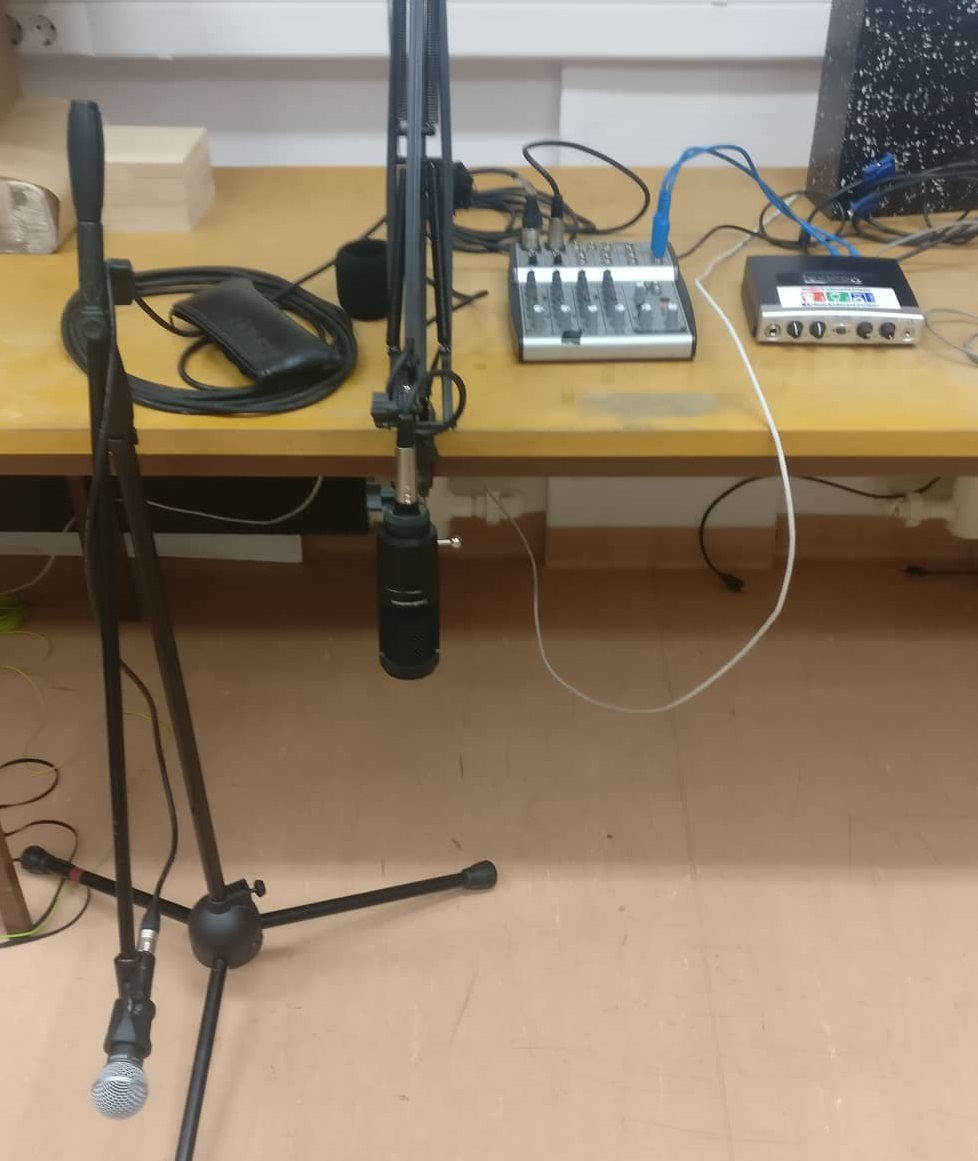
\includegraphics[width=0.6\textwidth]{img/recording_setup}
  \caption{Audio recording setup with two microphones, a mixer and an USB sound card}
  \label{fig:rec_setup}
\end{figure}

\subsubsection{Data preprocessing}
Each take was exported to an individual \verb+*.wav+ file with the naming scheme \verb+ID_shoeType_##.wav+.

\subsection{Model}
I choose \verb+InceptionV3+ as the basis for my model. The top part of the model was replaced with a dense feed forward network to classify the data into 6 classes. The model consisted of a flatten layer, two hidden layers with size 126 and 32, with ReLU activation functions and dropout with 0.5 probability. The output layer consisted of 6 neurons with a softmax function.

\subsection{Training}
I tried to follow the general steps of transfer learning on a CNN, but training the classification model on the bottleneck features of InceptionV3 with the ImageNet wights proved to be of little use: it was clear that the feature extraction needed for the spectrograms is different than what is used for normal photographs.

Still, ImageNet weights proved to be useful as a pretraining of the network??

\subsection{Hyper-parameter optimization}

\subsection{Results}

\section{Outlook, future plans}

\subsection{Figures}

\begin{figure}[ht]
  \centering
  \fbox{\rule[-.5cm]{0cm}{4cm} \rule[-.5cm]{4cm}{0cm}}
  \caption{Sample figure caption.}
\end{figure}

\subsection{Tables}

All tables must be centered, neat, clean and legible.  The table number and
title always appear before the table.  See Table~\ref{sample-table}.

This package was used to typeset Table~\ref{sample-table}.

\begin{table}[ht]
  \caption{Sample table title}
  \label{sample-table}
  \centering
  \begin{tabular}{lll}
    \toprule
    \multicolumn{2}{c}{Part}                   \\
    \cmidrule(r){1-2}
    Name     & Description     & Size ($\mu$m) \\
    \midrule
    Dendrite & Input terminal  & $\sim$100     \\
    Axon     & Output terminal & $\sim$10      \\
    Soma     & Cell body       & up to $10^6$  \\
    \bottomrule
  \end{tabular}
\end{table}



\subsubsection*{Acknowledgments}

Use unnumbered third level headings for the acknowledgments. All acknowledgments
go at the end of the paper. Do not include acknowledgments in the anonymized
submission, only in the final paper.

\section*{References}

References follow the acknowledgments. Use unnumbered first-level heading for
the references. Any choice of citation style is acceptable as long as you are
consistent. It is permissible to reduce the font size to \verb+small+ (9 point)
when listing the references. {\bf Remember that you can use more than eight
  pages as long as the additional pages contain \emph{only} cited references.}
\medskip

\small

[1] Alexander, J.A.\ \& Mozer, M.C.\ (1995) Template-based algorithms for
connectionist rule extraction. In G.\ Tesauro, D.S.\ Touretzky and T.K.\ Leen
(eds.), {\it Advances in Neural Information Processing Systems 7},
pp.\ 609--616. Cambridge, MA: MIT Press.

[2] Bower, J.M.\ \& Beeman, D.\ (1995) {\it The Book of GENESIS: Exploring
  Realistic Neural Models with the GEneral NEural SImulation System.}  New York:
TELOS/Springer--Verlag.

[3] Hasselmo, M.E., Schnell, E.\ \& Barkai, E.\ (1995) Dynamics of learning and
recall at excitatory recurrent synapses and cholinergic modulation in rat
hippocampal region CA3. {\it Journal of Neuroscience} {\bf 15}(7):5249-5262.

\end{document}
